% This LaTeX was auto-generated from MATLAB code.
% To make changes, update the MATLAB code and export to LaTeX again.

\documentclass{article}

\usepackage[utf8]{inputenc}
\usepackage[T1]{fontenc}
\usepackage{lmodern}
\usepackage{graphicx}
\usepackage{color}
\usepackage{hyperref}
\usepackage{amsmath}
\usepackage{amsfonts}
\usepackage{epstopdf}
\usepackage[table]{xcolor}
\usepackage{matlab}
\usepackage[paperheight=795pt,paperwidth=614pt,top=72pt,bottom=72pt,right=72pt,left=72pt,heightrounded]{geometry}

\sloppy
\epstopdfsetup{outdir=./}
\graphicspath{ {./project_one_v5_media/} }

\matlabmultipletitles

\begin{document}

\matlabtitle{\textbf{Project One: }\texttt{\textit{\textbf{Data Flow Modeling Using Matrix Theory}}}}

\matlabheading{\texttt{Applied Linear Algebra}  |  \textit{Student Name: }\texttt{\textit{Ryan Hatch}}\textit{  |  Date: }\texttt{\textit{10/4/24}}}


\begin{matlabcode}
%<><><><><><><><><><><><><><><><><><><><><><><><><><><><><><><><><><><><><><>
\end{matlabcode}


\label{T_B1FC42A4}
\matlabtitle{\textbf{Problem 1}}

\matlabheading{\textbf{Develop a system of linear equations for the network }by writing an equation for each router \texttt{(A, B, C, D, and E)}. }

\matlabheading{Make sure to write your final answer as \texttt{A}\texttt{\textbf{x}}\texttt{=}\texttt{\textbf{b}} where \texttt{A} is the \texttt{5x5} coefficient matrix, \texttt{\textbf{x}} is the \texttt{5x1} vector of unknowns, and \texttt{\textbf{b}} is a \texttt{5x1} vector of constants.}

\matlabheadingtwo{Solution - Define the data rates between routers:}

\begin{par}
\begin{flushleft}
\texttt{x1: From Router A to Router B}
\end{flushleft}
\end{par}

\begin{par}
\begin{flushleft}
\texttt{x2: From Router A to Router E}
\end{flushleft}
\end{par}

\begin{par}
\begin{flushleft}
\texttt{x3: From Router B to Receiver}
\end{flushleft}
\end{par}

\begin{par}
\begin{flushleft}
\texttt{x4: From Router E to Router D}
\end{flushleft}
\end{par}

\begin{par}
\begin{flushleft}
\texttt{x5: From Router C to Router D}
\end{flushleft}
\end{par}


\begin{par}
\begin{flushleft}
\textbf{The system of equations based on inputs and outputs for each router is:}
\end{flushleft}
\end{par}

\begin{par}
\begin{flushleft}
1. \texttt{Router A: x1 + x2 = 100}
\end{flushleft}
\end{par}

\begin{par}
\begin{flushleft}
2. \texttt{Router B: x1 = x3}
\end{flushleft}
\end{par}

\begin{par}
\begin{flushleft}
3. \texttt{Router C: x5 = 50}
\end{flushleft}
\end{par}

\begin{par}
\begin{flushleft}
4. \texttt{Router D: x4 + x5 = 120}
\end{flushleft}
\end{par}

\begin{par}
\begin{flushleft}
5. \texttt{Router E: x2 = x4}
\end{flushleft}
\end{par}


\begin{par}
\begin{flushleft}
\textbf{Defining the matrix A, vector x, and vector b:}
\end{flushleft}
\end{par}

\begin{par}
\begin{flushleft}
\texttt{A = [1  1  0  0  0;    -1  0  1  0  0;     0  0  0  0  1;     0  0  0  1  1;     0 -1  0  1  0];}
\end{flushleft}
\end{par}

\begin{par}
\begin{flushleft}
\texttt{x = ['x1'; 'x2'; 'x3'; 'x4'; 'x5'];}
\end{flushleft}
\end{par}

\begin{par}
\begin{flushleft}
\texttt{b = [100; 0; 50; 120; 0];}
\end{flushleft}
\end{par}


\begin{par}
\begin{flushleft}
\textbf{Code to display the matrix and constant vector:}
\end{flushleft}
\end{par}

\begin{matlabcode}
% Defining the coefficient matrix A and vector b for the system Ax = b
A = [1  1  0  0  0;  % Equation for Router A: x1 + x2 = 100
    -1  0  1  0  0;  % Equation for Router B: x1 = x3
     0  0  0  0  1;  % Equation for Router C: x5 = 50
     0  0  0  1  1;  % Equation for Router D: x4 + x5 = 120
     0 -1  0  1  0]; % Equation for Router E: x2 = x4

b = [100;  % Input to Router A
      0;   % Output from Router B to Receiver
      50;  % Input to Router C
      120; % Output from Router D to Receiver
      0];  % Output from Router E to Router D

% Display the coefficient matrix and constant vector
disp('Coefficient matrix A:');
\end{matlabcode}
\begin{matlaboutput}
Coefficient matrix A:
\end{matlaboutput}
\begin{matlabcode}
disp(A);
\end{matlabcode}
\begin{matlaboutput}
     1     1     0     0     0
    -1     0     1     0     0
     0     0     0     0     1
     0     0     0     1     1
     0    -1     0     1     0
\end{matlaboutput}
\begin{matlabcode}
disp('Constant vector b:');
\end{matlabcode}
\begin{matlaboutput}
Constant vector b:
\end{matlaboutput}
\begin{matlabcode}
disp(b);
\end{matlabcode}
\begin{matlaboutput}
   100
     0
    50
   120
     0
\end{matlaboutput}


\begin{matlabcode}
%<><><><><><><><><><><><><><><><><><><><><><><><><><><><><><><><><><><><><><>
\end{matlabcode}


\label{T_C0932C9D}
\matlabtitle{\textbf{Problem 2}}

\begin{par}
\begin{flushleft}
Use MATLAB to construct the augmented matrix [A \textbf{b}] and then perform row reduction using the rref() function. Write out your \textbf{reduced matrix and identify the free and basic variables of the system}.
\end{flushleft}
\end{par}

\label{H_2EAD55B4}
\matlabheadingtwo{Solution:}

\begin{matlabcode}
% Define the coefficient matrix A
A = [1,  1,  0,  0,  0;
    -1,  0,  1,  0,  0;
     0,  0,  0,  0,  1;
     0,  0,  0,  1,  1;
     0, -1,  0,  1,  0];

% Define the constants vector b
b = [100; 0; 50; 120; 0];

% Construct the augmented matrix [A | b]
AugmentedMatrix = [A b];

% Perform row reduction using rref()
ReducedMatrix = rref(AugmentedMatrix);

% Display the reduced matrix
disp('Reduced Augmented Matrix:');
\end{matlabcode}
\begin{matlaboutput}
Reduced Augmented Matrix:
\end{matlaboutput}
\begin{matlabcode}
disp(ReducedMatrix);
\end{matlabcode}
\begin{matlaboutput}
     1     0     0     0     0    30
     0     1     0     0     0    70
     0     0     1     0     0    30
     0     0     0     1     0    70
     0     0     0     0     1    50
\end{matlaboutput}

\begin{par}
\begin{flushleft}
\textbf{Reduced Augmented Matrix:}
\end{flushleft}
\end{par}

\begin{par}
\begin{flushleft}
1 0 0 0 0 30
\end{flushleft}
\end{par}

\begin{par}
\begin{flushleft}
0 1 0 0 0 70
\end{flushleft}
\end{par}

\begin{par}
\begin{flushleft}
0 0 1 0 0 30
\end{flushleft}
\end{par}

\begin{par}
\begin{flushleft}
0 0 0 1 0 70
\end{flushleft}
\end{par}

\begin{par}
\begin{flushleft}
0 0 0 0 1 50
\end{flushleft}
\end{par}

\begin{par}
\begin{flushleft}
\textbf{Identification of Variables: }\textit{All variables x1, x2, x3, x4, x5 are basic variables.} 
\end{flushleft}
\end{par}

\begin{par}
\begin{flushleft}
There are also no free variables and the system has a unique solution.
\end{flushleft}
\end{par}


\begin{matlabcode}
%<><><><><><><><><><><><><><><><><><><><><><><><><><><><><><><><><><><><><><>
\end{matlabcode}


\label{T_9BF65707}
\matlabtitle{\textbf{Problem 3}}

\begin{par}
\begin{flushleft}
Use MATLAB to \textbf{compute the LU decomposition of A}, i.e., find A = LU. For this decomposition, find the transformed set of equations L\textbf{y} = \textbf{b}, where \textbf{y} = U\textbf{x}. Solve the system of equations L\textbf{y} = \textbf{b} for the unknown vector \textbf{y}.
\end{flushleft}
\end{par}

\label{H_EA39FD3F}
\matlabheadingtwo{Solution:}

\begin{matlabcode}
% Perform LU decomposition
[L, U] = lu(A);

% Display L and U matrices
disp('L matrix:');
\end{matlabcode}
\begin{matlaboutput}
L matrix:
\end{matlaboutput}
\begin{matlabcode}
disp(L);
\end{matlabcode}
\begin{matlaboutput}
     1     0     0     0     0
    -1     1     0     0     0
     0     0     0     0     1
     0     0     0     1     0
     0    -1     1     0     0
\end{matlaboutput}
\begin{matlabcode}
disp('U matrix:');
\end{matlabcode}
\begin{matlaboutput}
U matrix:
\end{matlaboutput}
\begin{matlabcode}
disp(U);
\end{matlabcode}
\begin{matlaboutput}
     1     1     0     0     0
     0     1     1     0     0
     0     0     1     1     0
     0     0     0     1     1
     0     0     0     0     1
\end{matlaboutput}
\begin{matlabcode}

% Solve L * y = b for y
y = L \ b;

% Display the vector y
disp('Solution vector y:');
\end{matlabcode}
\begin{matlaboutput}
Solution vector y:
\end{matlaboutput}
\begin{matlabcode}
disp(y);
\end{matlabcode}
\begin{matlaboutput}
   100
   100
   100
   120
    50
\end{matlaboutput}

\begin{par}
\begin{flushleft}
The \texttt{\textit{lu()}} function solves for the \texttt{LU} decomposition of \texttt{matrix A.}
\end{flushleft}
\end{par}

\begin{par}
\begin{flushleft}
\textbf{L} is a lower triangular matrix, and \textbf{U} is an upper triangular matrix.
\end{flushleft}
\end{par}

\begin{par}
\begin{flushleft}
I solved \texttt{\textbf{Ly = b}} using forward substitution.
\end{flushleft}
\end{par}


\begin{matlabcode}
%<><><><><><><><><><><><><><><><><><><><><><><><><><><><><><><><><><><><><><>
\end{matlabcode}


\label{T_9BF65707}
\matlabtitle{\textbf{Problem 4}}

\begin{par}
\begin{flushleft}
\textbf{Compute the inverse }of U using the inv() function using MATLAB.
\end{flushleft}
\end{par}

\label{H_EA39FD3F}
\matlabheadingtwo{Solution:}

\begin{matlabcode}
% Compute the inverse of U
U_inv = inv(U);

% Display the inverse of U
disp('Inverse of U:');
\end{matlabcode}
\begin{matlaboutput}
Inverse of U:
\end{matlaboutput}
\begin{matlabcode}
disp(U_inv);
\end{matlabcode}
\begin{matlaboutput}
     1    -1     1    -1     1
     0     1    -1     1    -1
     0     0     1    -1     1
     0     0     0     1    -1
     0     0     0     0     1
\end{matlaboutput}

\begin{par}
\begin{flushleft}
The \texttt{inv()} function computes the inverse of a matrix.
\end{flushleft}
\end{par}

\begin{par}
\begin{flushleft}
Finding out the solution to \texttt{\textbf{U\textasciicircum{}-1}} helped me to find \texttt{\textbf{x}} again in the future.
\end{flushleft}
\end{par}


\begin{matlabcode}
%<><><><><><><><><><><><><><><><><><><><><><><><><><><><><><><><><><><><><><>
\end{matlabcode}


\label{T_9BF65707}
\matlabtitle{\textbf{Problem 5}}

\begin{par}
\begin{flushleft}
\textbf{Compute the solution to the original system of equations }by transforming \textbf{y }into \textbf{x}, i.e., compute \textbf{x} = inv(U)\textbf{y}.
\end{flushleft}
\end{par}

\label{H_EA39FD3F}
\matlabheadingtwo{Solution:}

\begin{matlabcode}
% Compute the solution vector x
x = U_inv * y;

% Display the solution vector x
disp('Solution vector x:');
\end{matlabcode}
\begin{matlaboutput}
Solution vector x:
\end{matlaboutput}
\begin{matlabcode}
disp(x);
\end{matlabcode}
\begin{matlaboutput}
    30
    70
    30
    70
    50
\end{matlaboutput}

\begin{par}
\begin{flushleft}
Multiplying \texttt{\textbf{U\textasciicircum{}-1}} and \texttt{y} gave me the solution \texttt{\textbf{x}}.
\end{flushleft}
\end{par}

\begin{par}
\begin{flushleft}
This technically solves the original system \texttt{\textbf{Ax = b}}.
\end{flushleft}
\end{par}


\begin{matlabcode}
%<><><><><><><><><><><><><><><><><><><><><><><><><><><><><><><><><><><><><><>
\end{matlabcode}


\label{T_9BF65707}
\matlabtitle{\textbf{Problem 6}}

\begin{par}
\begin{flushleft}
\textbf{Check answer for }$x_1$ \textbf{using Cramer’s Rule.} Use MATLAB to compute the required determinants using the det() function. 
\end{flushleft}
\end{par}

\label{H_EA39FD3F}
\matlabheadingtwo{Solution:}

\begin{matlabcode}
% Compute the determinant of A
detA = det(A);

% Replace the first column of A with b to form A1
A1 = A;
A1(:,1) = b;

% Compute the determinant of A1
detA1 = det(A1);

% Compute x1 using Cramer's Rule
x1 = detA1 / detA;

% Display the computed x1
disp('x1 computed using Cramer''s Rule:');
\end{matlabcode}
\begin{matlaboutput}
x1 computed using Cramer's Rule:
\end{matlaboutput}
\begin{matlabcode}
disp(x1);
\end{matlabcode}
\begin{matlaboutput}
   30.0000
\end{matlaboutput}

\begin{par}
\begin{flushleft}
\textbf{Cramer's Rule:} \texttt{xi = det(Ai) / det(A) - } where \texttt{Ai} is \texttt{A} with its \texttt{i-th} column replaced by \texttt{b.}
\end{flushleft}
\end{par}

\begin{par}
\begin{flushleft}
I solved \texttt{det(A)} and \texttt{det(A1)} in order to find \texttt{x1.}
\end{flushleft}
\end{par}


\begin{matlabcode}
%<><><><><><><><><><><><><><><><><><><><><><><><><><><><><><><><><><><><><><>
\end{matlabcode}


\label{T_9BF65707}
\matlabtitle{\textbf{Problem 7}}

\matlabheadingthree{Solution for the system of equations in the third column so it can be easily compared to the maximum capacity in the second column. }

\matlabheadingthree{In the fourth column of the table, provide recommendations for how the network should be modified based on your network throughput analysis findings. The modification options can be \texttt{No Change}, \texttt{Remove Link}, or \texttt{Upgrade Link.} In the final column, explain how you arrived at your recommendation.}


\label{H_EA39FD3F}
\matlabheadingtwo{Solution:}

\begin{par}
\begin{center}
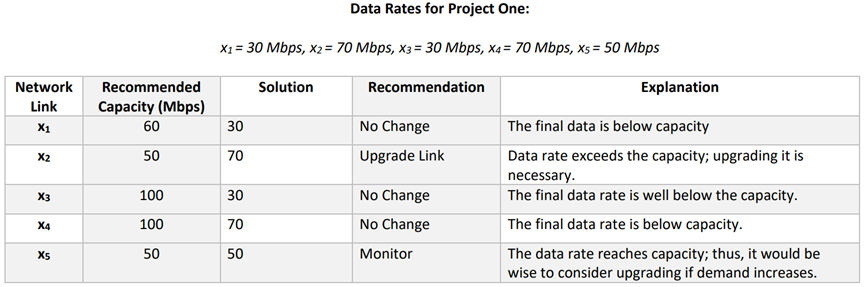
\includegraphics[width=\maxwidth{86.70346211741094em}]{image_0}
\end{center}
\end{par}

\begin{par}
\begin{flushleft}
\textit{By modeling the network as a system of linear equations and then applying matrix techniques to solve them, I was able to find out what the data rates for each link in the network are. Using the tools from MATLAB I was able to perform tasks like row reduction, LU decomposition, and I also applied Cramer's Rule to verify the solutions. In the final result, I then gave recommendations that were based on the data rates to make sure that the network operates at the most optimal rate without over working or exceeding any link capacities.}
\end{flushleft}
\end{par}


\begin{matlabcode}
%<><><><><><><><><><><><><><><><><><><><><><><><><><><><><><><><><><><><><><>
\end{matlabcode}

\end{document}
